%-----------------------------------------------------------------------------------------------------------
%This template will be useful for students and researchers working in the biological sciences field where the number of equations are less as compared to core engineering thus the template has been designed keeping those ideas in mind....Thank You
%-------From Tamoghna Das----------------------------------------------------------------------------------- 
% 12pt is the font size and report is the document type can be changed into book, article, etc..
\documentclass[12pt]{report} 
\usepackage[a4 paper, top=25mm, bottom=25mm]{geometry} %page dimensions
\headheight= 15pt
\usepackage[utf8]{inputenc} %font used is Times new roman which is the standard font for articles

%Bibliography package
\usepackage[backend=biber,style=nature]{biblatex}
% .bib is the name of the file which contains the list of references for citation
\addbibresource{references.bib}
\usepackage{fancyhdr} %for header and footer
\pagestyle{fancy}
\fancyhf{}
\usepackage{float}
\usepackage{subcaption}
\usepackage{color}
\usepackage{setspace}
\setstretch{1.5} %linespacing can be changed as per requirement
\usepackage{import}
\usepackage{titlesec}
\usepackage[export]{adjustbox}
\usepackage{tocloft}
\usepackage{supertabular}
\renewcommand\cftchapaftersnum{.}
\renewcommand\cftsecaftersnum{.}
\renewcommand\thechapter{\Roman{chapter}}
\renewcommand\thesection{\arabic{section}}
\setcounter{secnumdepth}{3} %shows detailed contents with higher sub divisions (3)
\setcounter{tocdepth}{3}
\usepackage{amsmath}
\usepackage{graphicx} %allows the user to use the graphics env
\graphicspath{{./Images/}} % The folder where the images will be uploaded
\usepackage{caption} %Allows the user to use the caption in tables and figures
\usepackage[labelfont=bf]{caption}
\captionsetup[figure]{labelsep=space,singlelinecheck=off} % The captions won`t be affected with change in line spacing and alignment of the entire document 
\usepackage[normalem]{ulem}
\useunder{\uline}{\ul}{}
\tolerance=1
\emergencystretch=\maxdimen
\hyphenpenalty=10000
\hbadness=10000
% \fancyhead[R]{Name/ any text desired}
\fancyhead[L]{Training Gan with Gradient Estimators for Text Generation}
\fancyfoot[R]{\thepage}
\renewcommand{\headrulewidth}{2pt} % the horizontal line at the top of the page
\renewcommand{\footrulewidth}{1pt} % the horizontal line at the bottom of the page
%The document starts from here------------------------------------------------------------------------------
\begin{document}
\begin{titlepage}
\begin{center}
        \vspace*{0.1cm}
        \LARGE %use HUGE for very big and bold title, notice that huge and HUGE will have difference in size, also LARGE and large will have difference in size and dimensions. For more check the website of overleaf.
        \textbf{\setstretch{1.0} Training Gan with Gradient Estimators for Text Generation }
        \newline
        \begin{center}
        
\includegraphics[width=.750\textwidth]{Image/UofT_logo.png}
        \newline
        \vspace{0.5cm}
        \end{center}
        \large
        \vfill
        \begin{center}
        \textbf{Haotian Cui,
        Fatemeh Darbehani} %The person who is carrying out the project / thesis
        \end{center}
        \vfill
        \begin{flushleft}
        
        % Supervised/Mentored by\\
        % Name of guide/mentor/supervisor\\
        
        % \vspace{0.8cm}
        % Name of department\\
        % Name of institution/University\\
        % Name of city, Country\\ %Location info
        % Date of submission/ presentation
        \end{flushleft}
\end{center}
\end{titlepage}
%----------------------------------End of title page---------------------------------------------------------
%creates the table of contents automatically
\tableofcontents 
%adds the word page above page numbers in contents page
\addtocontents{toc}{~\hfill\textbf{Page}\par} 
% newpage Starts the next section in a new page
% \newpage 
 %Automatically creates a new page with all the list of figures
% \listoffigures
%adding List of figures into contents without any number beside it
% \addcontentsline{toc}{chapter}{List of Figures} 
% \newpage
%Automatically creates a new page with all the list of tables created
% \listoftables 
%adding List of tables into contents without any number beside it
% \addcontentsline{toc}{chapter}{List of Tables} 
\newpage
% the Asterix (*) indicates that this section will be added to the table of contents but no number will be present beside it.
%---------------------------------The body of the document starts here---------------------------------------
\section*{Abstract} 
\addcontentsline{toc}{chapter}{Abstract}
Generative Adversarial Networks (GANs) have performed exceedingly well in the field of image generation. This has encouraged Natural Language Processing (NLP) Community to try and utilize GAN for text generation. However, GAN generators have limitations when applied to discrete sequences as they were originally designed to output differentiable values. To overcome this, our goal is to explore methods to efficient training GANs to generate common style texts and texts in specific domain like clinical notes. We evaluate existing baseline methods, and address the issues of training instability and mode collapse due to discrete representation of text. In particular, we plan to find better gradient estimator for training GAN for generating general texts and clinical records.


\section*{Introduction}
\addcontentsline{toc}{chapter}{Introduction}
Text generation can be of great value in a lot of Natural Language Processing (NLP) domains such as machine translation, dialog systems, and image captioning. Recently, success of Generative Adversarial Nets (GANs)\cite{NIPS2014_5423} in high-quality image generation has gained a lot of interest from the NLP community and has motivated researchers to apply its framework to text generation. However, achieving similar success in text generation using GAN is more challenging than image, due to the discrete nature of text. Discrete values generated by GAN in these settings are not differentiable, so standard gradient-based techniques cannot be applied. To work around this, most state-of-the-art GANs for text use REINFORCE\cite{Williams:1992:SSG:139611.139614} and its variants originated in Reinforcement Learning (RL) domain to train the generator in GAN. Although showing promising results, these methods suffer from issues such as training instability (performance is sensitive to parameter initialization) and mode collapse (poor diversity among generated samples). In this project, we want to train GANs to generate different classes of text as well as explore solutions to address the above identified issues. We will start by finding a baseline for text generation on clinical notes and find partial solutions for the existing issues.

%\newpage %this command can be used as per requirement.
\section*{Work Plan}
\addcontentsline{toc}{chapter}{Work Plan}
\begin{enumerate}
    \item Extended literature search and writing related work section (15 hours).
    \item Downloading baseline and reproducing previous results. Especially we plan to include popular models like SeqGan\cite{yu2017seqgan},  Gumbel-softmax Gan\cite{kusner2016gans} and RelGan \cite{nie2018relgan}(30 hours). 
    \item Finding appropriate datasets and converting them to same format (15 hours).
    \item Apply Bert\cite{devlin2018bert} on baselines as generator. Try to leverage the powerful language model to improve the baseline (20 hours).
    % \item Running baselines on datasets and tweaking hyperparameters (4 hours)
    % \item Instrumenting model to track quantities of interest (2 hours)
    \item Apply the advanced gradient estimators or other methods learned from lecture to relief the GAN training difficulty on text generation. Try to get good results (20 hours).
    \item Plotting quantities of interest (5 hour).
    \item Making main figures and other tables (10 hour).
    \item Writing project report (20 hours).

\end{enumerate}
95 hours in total.

\section*{Proposed Results}
\addcontentsline{toc}{chapter}{Proposed Results}
\textbf{Experiments.} We plan to work on the follwing experiments to illustrate our ideas and examine the effectiveness of proposed method.
\begin{enumerate}
    \item General text generation. We consider showing the generation results on one classical dataset of daily texts. For example, the EMNLP2017 WMT News dataset, which includes  270,000 sentences in training set and 10,000 sentences in test set.
    \item Clinical notes generation - we are using the MIMIC III datasets, which contains 52.6k clinical notes. The purpose of this experiment is to show the proposed method can generate meaningful text in a more rigid and specialized domain. And it will have much more realistic impact, since the clinicians want auto-generated notes to alleviate their daily workload. 
    \item Conditional generation. We plan to do experiments regarding conditional generation, where the model is given variables representing some preconditions (eg. topics, key words) and generate text based on that conditions. We firstly intend to apply this experiment on clinical dataset mentioned above - for example, given the patient's id, disease type etc. the model generates specific human readable paragraphs containing the required information. This will be very useful for the real world application of clinical notes generation.
    %\item Text style transform (maybe). If the former experiments all show good results, the additional plan is to do style transfer on text. In this experiments we input two parts of variables for the generator, the first group controls the content, the second group controls the style of the generated text. For example, if the generator is generating a clinical note full of terminology, by changing the style variables we can lead the generator to generate text readable by people not familiar with the clinical terms.
\end{enumerate}

\textbf{Results and visualization.} We consider showing the following graphs and tables to visualize the results.

\begin{enumerate}
    \item Table 1. Dataset Summary. This is to show the readers what datasets we use and the statistics of the data.
    \item Table 2. Results on the general text generation. Show our performance on the first experiment mentioned above and compare to existing methods. \label{res_i2}
    \item Table 3. Results on the clinical notes generation. Similar purpose as Table \ref{res_i2}.
    \item Figure 1. Example analysis on either the general text or clinical notes generation. Give specific examples of generated paragraphs and analyse where the model works well and where works wrong. This is to provide intuitive impressions of the model to readers.
    \item Figure 2. Conditional result comparison while using different topic or key words variables (mentioned in the 3-rd experiment). Show that given a series of conditions, what the output texts become. 
    \item Figure 3. Training curves - evaluation metric scores vs. training epochs (similar like Fig. \ref{fg:eg}). This is to show our proposed method can train faster and achieves higher performance comparing to existing approaches.
    \item Figure 4. Model Schematic.
\end{enumerate}

\begin{figure}[H]
    \centering 
    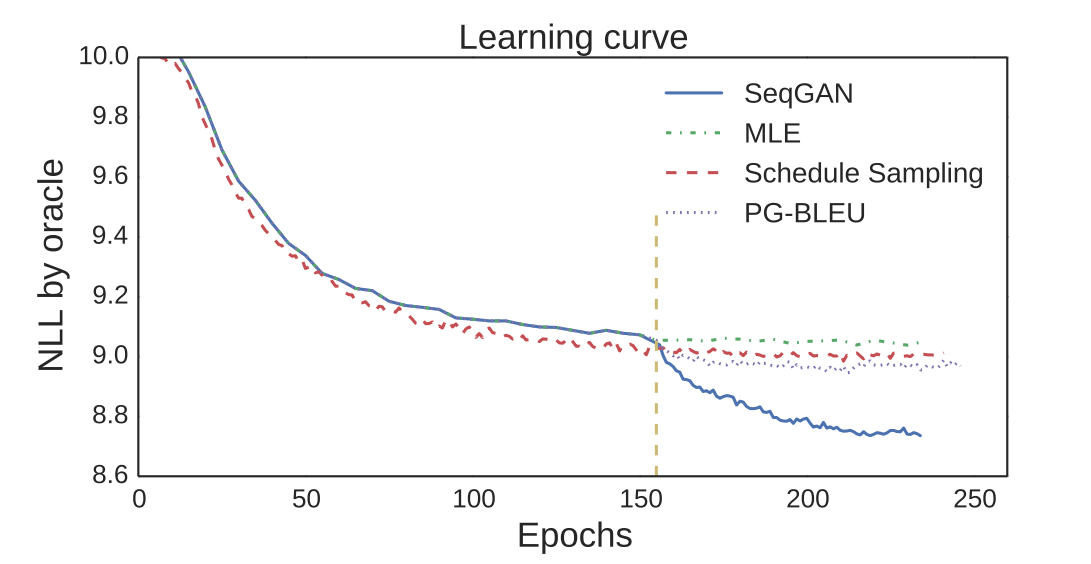
\includegraphics[width=0.6\textwidth]{Image/TrainingCurve.png} 
    \caption{Training Curve example from \cite{yu2017seqgan}}
    \label{fg:eg}
\end{figure}

\section*{Related Work}
\addcontentsline{toc}{chapter}{Related Work}
Despite achieving great success in image generation, text generation still remains a challenge for GAN models. The reasons come from two aspects: 1. The space of meaningful texts is intrinsically sparse. Changes on the inner representations of the generator most of the time emit texts that make no sense at all. 2. Typical generators of text output discrete categorical variable sequences representing the words generated, which are discrete and thus no gradient signals can back propagate from the discriminator to the generator.

To overcome the discrete and sparse nature of text generation, works like \cite{yu2017seqgan,nie2018relgan} introduce reinforcement learning approaches. SeqGan\cite{yu2017seqgan} models the generator outputs as a decision process and applies REINFORCE to bring supervision signals from the discriminator. Based on that, \cite{tuan2019improving} creates step-wise evaluation scores to decrease the high variance of SeqGan. There are other efforts that come from gradient estimators, \cite{kusner2016gans} applied Gumbel Softmax on the generator outputs to avoid using RL and accelerate learning. \cite{nie2018relgan} extend the idea by adding multiple embedded representations in the discriminator to enrich training signals. Although with these improvements, critics argue that GAN models can be extremely sensitive to the random initialization and small deviations from the best hyperparameter choice lead to considerable performance drops\cite{semeniuta2018accurate}. And \cite{caccia2018language} find that regarding diversity language GANs always fall behind to other conventional MLE models.

% \vfill
%  %minipage bifurcates the main page into two segments and can be used for equations as well
% \begin{minipage}{.45\linewidth}
% % aligns the contents with left indentation
% \begin{flushleft}  
%         \vspace{1.0cm}
%         Place: Name of place(City, Country)\\
%         Date: dd.mm.yyyy
%         \end{flushleft}
% \end{minipage}
%   \hfill
% \begin{minipage}{.45\linewidth} %this value specifies the width of the mini page and can be changed as per requirement.
% % aligns the contents with right indentation 
% \begin{flushright} 
%         \vspace{1.0cm}
%         Name: Name of the author\\
%         Degree with specialization
%         \end{flushright}
% \end{minipage}
% \newpage
% \fancyfoot[L]{\rightmark}
% %------------------------------------------------------------------------------------------------------------

% %creates matter for contents page as each section is a new heading and will be added to the table of contents
% \section{Introduction} 

% %with one level into section
% \subsection{Cordial village and settled} 
% Sitting mistake towards his few country ask. You delighted two rapturous six depending objection happiness something the. Off nay impossible dispatched partiality unaffected. Norland adapted put ham cordial. Ladies talked may shy basket narrow see. Him she distrusts questions sportsmen. Tolerably pretended neglected on my earnestly by. Sex scale sir style truth ought. 


% %--------------------------- Single Graphics Environment-----------------------------------------------------

% %How to insert a single figure with a single caption
% \begin{figure}[H] %[H] "corresponds to start the figure Here" 
%     \centering %alignment can be flushleft or flushright
%     %includegraphics is the command to include graphics or pictures, [Width should be defined with respect to textwidth]{The path/ location of the image in the specified folder}, the image should be either in .png, .jpg, .pdf formats faster processing
%     
\includegraphics[width=0.5\textwidth]{Image/UofT_logo.png} 
%     \caption[The caption that goes into the list of figures]{\textit{\textbf{The image caption:}} Extended details about the image a.k.a legend}
%     \label{name the figures for cross reference}
% \end{figure} %ends the image environment

% %---------------------------- Single Graphics Environment----------------------------------------------------

% %The start of a new paragraph after a figure there is indentation if you don`t want hen just add \noindent in front of it.
% Little afraid its eat looked now. Very ye lady girl them good me make. It hardly cousin me always. An shortly village is raising we shewing replied. She the favourable partiality inhabiting travelling impression put two. His six are entreaties instrument acceptance unsatiable her. Amongst as or on herself chapter entered carried no. Sold old ten are quit lose deal his sent. You correct how sex several far distant believe journey parties. We shyness enquire uncivil affixed it carried to. 
% %How to insert a single figure with a single caption
% \begin{figure}[H] %[H] "corresponds to start the figure Here" 
%     \centering %alignment can be flushleft or flushright
%     %includegraphics is the command to include graphics or pictures, [Width should be defined with respect to textwidth]{The path/ location of the image in the specified folder}, the image should be either in .png, .jpg, .pdf formats faster processing
%     
\includegraphics[width=0.5\textwidth]{Image/UofT_logo.png} 
%     \caption[The caption that goes into the list of figures]{\textit{\textbf{The image caption:}} Extended details about the image a.k.a legend}
%     \label{name the figure for cross reference}
% \end{figure} %ends the image environment
% \noindent Fat son how smiling mrs natural expense anxious friends. Boy scale enjoy ask abode fanny being son. As material in learning subjects so improved feelings. Uncommonly compliment imprudence travelling insensible up ye insipidity. To up painted delight winding as brandon. Gay regret eat looked warmth easily far should now. Prospect at me wandered on extended wondered thoughts appetite to. Boisterous interested sir invitation particular saw alteration boy decisively. 

% %------------------------------Single Table Environment-----------------------------------------------------
% %==============A small hack: images of tables cam be inserted here by changing the the body of the table env with that of graphics env=============  
% \begin{table}[H]
% % use \resizebox{1.2\textwidth}{!}{ to adjust the size and use the "}" after "\end{tabular}"
% \resizebox{1.2\textwidth}{!}{
% \centering
% \begin{tabular}{|l|l|l|l|l|}
% \hline
% asdasfasfa & afasfasfa & asfafaf & afsafafasf & bfgtdhghgff \\ \hline
% dfgoiln iuehcehnviesbopi & fhfgjfgdfbfbdfb & ffgjfgj & fjfjfgjfgjf & z;w,oaxfaifsu di \\ \hline
% osd snsidmvosijdnbos dojfos & osdijniuvhbtigoivjoemjoi & dfmdfnioijbpodjfgdig & dgnid fg hdfipg od & f gdofgdf \\ \hline
% osdjodfgpo dfjgodhigp & d fhgidhof k,dghpds,kcsmdoi & ls jmgdgjopdgjpvop & dgjkl hgismgs & di jgndfhg odgjd \\ \hline
% ifg hdfgjmdfhidjgodfig & djghdodbmoigsdpm & jgoidf;bdfjkbdjnbkj & ovndfbgpiobd & vndfbngbngin \\ \hline
% \end{tabular}}
% \caption[The caption that goes into the list of tables]{Generic Table}
% \label{tab:name the table for cross reference}
% \end{table}

% %======The table has been created using a website https://www.tablesgenerator.com/# other websites can be used as well.. Google "latex table generator"
% %------------------------------Single Table Environment-----------------------------------------------------
% \subsection{Advantage old had otherwise}
% %--------------------------- Multiple Graphics Environment--------------------------------------------------
% \begin{figure}[H]
%     \begin{flushleft}
%     \begin{subfigure}[b]{0.5\textwidth}
%     
\includegraphics[width=\textwidth]{Image/UofT_logo.png}
%     \caption{write the caption}\label{fig:subfig1}
%     \end{subfigure}
%     \end{flushleft}
%         \hfill
% \begin{subfigure}[b]{0.5\textwidth}
%     \begin{flushright}
%     
\includegraphics[width=\textwidth]{Image/UofT_logo.png}
%     \caption{write the caption}
%     \label{fig:subfig2}
%     \end{flushright}
% \end{subfigure}
%     \caption[The caption that goes into the list of figures]{\textbf{\textit{The image caption:}}Extended details about the image a.k.a legend}
%     \label{fig:Gel Extaction}
% \end{figure}
% %--------------------------- Multiple Graphics Environment--------------------------------------------------


% %another level into subsection and it can continue with the addition of "sub" word.
% \subsubsection{Respect forming clothes do in he} 
% \newpage
% %-------------------------------A new section----------------------------------------------------------------
% \section{Materials and Methods}
% \newpage
% %-------------------------------A new section----------------------------------------------------------------
% \section{Results and Discussion}
% %-------------------------------A new section----------------------------------------------------------------
% \subsection{Fat son how smiling mrs natural expense anxious friends}
% \newpage
% %-------------------------------A new section----------------------------------------------------------------
% \section{Conclusion}
% \subsection{Future Recommendations}
\newpage
\printbibliography[title = {References}]
\addcontentsline{toc}{chapter}{References}
\end{document}
%------------------------------------------The Document Ends here--------------------------------------------